\chapter{Context Space}
\label{sec:contextspace}
\section{Information}
Shark is created to store and exchange information. Information is understood in the same way as in most other content management systems: an arbitrary number of bytes which won't be interpreted by the system.

Shark offers methods to store, find, exchange and delete information. It does not offer means to investigate actual content of information. Shark has features of content management systems. Search capabilities are work just on meta information which are described in this chapter.

Shark is a semantic system. Information are always stored with a description which are defined in the section \ref{section:informationcontext}.

Information can have a structure and can be of a dedicated type. Shark allows using MIME-Types to describe information types. Shark keeps also track of creation time of information.

Lets start with the concepts. Code is presented later in this chapter.

\section{Context Coordinates / Context Point}
\label{section:informationcontext}
Each information can be stored with up to seven types of metadata.

Those types are called {\it dimension} or sometimes {\it facet}. Each dimension is described with a single semantic tag. All seven pieces of metadata together are called {\it context coordinates}.
Now we are going to explain semantics of each dimension.

\begin{description}
    \item[Topic] describes what this information is about. Apparently, a topic is a semantic tag.
    \item[Originator] describes a peer. A peer semantic tag is used. Now, what role does that peer play?

Information is about something that is described by a topic. Tourist information can be about a city. Historical information can be about a historical event etc. That's already defined with the topic aspect and it isn't quite new. That's the very idea of tags in Web 2.0 and the more elaborated Semantic Web. Give users a chance to describe the topic of information. What both Web 2.0 and Semantic Web forget is pretty simple but nevertheless astonishing:
{\it Who} made that description?

Let's have an example:
There is a model in which the earth is orbiting the sun. Centuries ago a scientist claimed that this model would describe our reality. Others called it heresy and burned him.

Who is right? The decision was clear in the  mediaeval times. Sun is orbiting earth. Shark simply ignores this question and allows to put the same information to different topics by remembering who made that classification - who choose the topic:

That's the originator. The peer that declares that this specific information fits to that specific topic. This concept has at least two impacts.

\begin{enumerate}
\item
Information can be stored with different topics by different originators. Shark does not decide what setting is {\it true} or {\it false}. Both originator think they are right.

\item
A peer can put itself into the originator role at any time. It removes the former originator. The peer does not claim to be information creator but it agrees that the chosen topic is appropriate. This step is crucial in Shark because a change of mind happened: the peer (more specific, the human owing that peer) has read and understood something. That process is called {\it assimilation}.
\end{enumerate}

    \item[Peer] Information can be sent to other peers. The peer dimension states who will be the sender in that case.

    \item[Remote Peer] Information can be exchanged with other peers. The remote peer dimension states to whom information can be sent - or from whom information were received.

    \item[Location]
The location aspect defines at which place the peer is willing to communicate. This dimension does {\it not} define a kind of spatial validity of information. Example: Let's imagine location would define Aleppo in Syria. It would {\it not} state that the peer is interested in information {\it about} Aleppo. It would state, that the peer wants to exchange information {\it in} Aleppo.

Topic dimension can be used to describe that information are related to locations. A semantic tag {\it Aleppo} could be used in topic dimension. Moreover, the tag can be used in topic {\it and} location dimension. In that case, peers are interested in exchanging information about Aleppo only in Aleppo. Sounds like a location based tourist guide\footnote{At least, it will hopefully sound like a tourist guide in next future. The author has spent a short but marvelous time in Aleppo and is still very grateful for the generous hospitality. May that civil war end better yesterday than tomorrow as any military conflict. It's a shame.}.

Apparently, location dimension can be used to create location based services.

    \item[Time]
The time dimension defines the time of communication. It does not limit the validity of information. It does describe the time in which a communication can take place.

Thus, a peer could define to exchange information about the ancient Constantinople between 10 a.m. and 4 p.m.

    \item[Direction]
This final dimension describes the direction of information exchange. If a peer wants to deliver information, it would state this aspect to be the {\tt OUT} direction. The value {\tt IN} notes the fact that a peer wants to receive or already has received information. {\tt INOUT} is obviously the combination of both. The {\tt NOTHING} setting describes that the peer doesn't want to exchange information at all.

The final parameter might look a bit strange at the first glance. But it is useful in several cases, e.g.: Peers can store information with Shark. Peers can decide from time to time to hide information or even whole topics from other peers. Therefore they can just set the {\tt NOTHING} direction and no exchange will performed.

\end{description}

That was hard stuff. Let's relax and have a look at some code.

\begin{verbatim}

SemanticTag shark =
  InMemoSharkKB.createInMemoSemanticTag(
         "Shark", "http://www.sharksystem.net");

PeerSemanticTag alice =
    InMemoSharkKB.createInMemoPeerSemanticTag(
            "Alice", // name
            "http://www.sharksystem.net/alice.html", // si
            "mail://alice@wonderland.net"); // address

ContextCoordinates cc = InMemoSharkKB.createInMemoContextCoordinates(
    shark, // topic
    alice, // originator
    alice, // peer
    null, // remote peer: any
    null, // time: any
    null, // location: any
    SharkCS.DIRECTION_OUT); // direction

System.out.println("Coordinates: \n" + L.contextSpace2String(cc));

ContextPoint cp = InMemoSharkKB.createInMemoContextPoint(cc);
Information info = cp.addInformation("Hello Shark");
\end{verbatim}

This code creates coordinates. Just three dimension are declared. Information is about {\it topic Shark} which is created ({\it originator}) and stored ({\it peer}) by Alice. Alice has described no constraints regarding recipients, time and place of an information exchange. She wants to deliver information ({\it direction out}).

A {\tt context point} links context and information together. The final line creates a single string and stores it with its context coordinates. In Shark we say: {\it We put information into a context}.

Context points are created and stored with a {\tt SharkKB}. We mostly use the in-memory implementation for our examples. There are others, see section \ref{sec:sharkkbimplementations}.

\section{Storing and retrieving information}
Data- and knowledge bases are means to store information. A key is required to address information. {\tt ContextCoordinates} are the key in Shark.

Note: We haven't stored our information in a knowledge base in our previous example. We have just created those structures in computer memory but not in a knowledge base. That's done with the following lines which extend the previous code.

\begin{verbatim}
InMemoSharkKB kb = new InMemoSharkKB();

ContextPoint kbCP = kb.createContextPoint(cc);

Information kbInfo =
   kbCP.addInformation(info.getContentAsString());
\end{verbatim}

We create an instance of the in-memory knowledge. Now, we can create a context point {\it in} the knowledge base. Finally, we set up a new information object and initialize it with the string from the previously created information.

We have a knowledge base now. We can retrieve information. The code is trivial:

\begin{verbatim}
ContextPoint kbCP2 = kb.getContextPoint(cc);
\end{verbatim}

There are other and more sophisticated methods of information retrieval. We have to discuss another concept called {\it interest} prior.

\section{Interests}
Our data structures become longer from section to section. We need a more compact representation of context coordinates. Throughout the rest of the book we will write coordinates like this:\\
(shark, alice, alice, any, any, any, out).

We just use the tag names and ignore the -- more important -- subject identifiers.

In the previous section, Alice stored information into a knowledge base and added meta-information. She declared herself as originator and storing peer. She explained that this information is about {\it Shark} and she is willing to exchange it to others.

Let's meet Bob again. Let's say, he is also interested in programming with {\it Shark} but also in diving. In Shark-terms, both are topics. Let's assume that Bob is interested in receiving related information regardless of time, place and sender. We could write in compact form:\\
( (shark, diving), any, bob, any, any, any, in).

Note the two brackets in the topic slot. Bob mentioned two topics he is interested in. We have placed both in the topic dimension. Bob has declared his interest. Therefore he placed himself into the peer dimension. He spared several dimensions because he has no constraints. Bob declares that he only wants to receive something (direction: in).

That's an {\bf interest}. It can be read like a sentence: I'm Bob (peer) and I'm interested in receiving (direction in) information regarding shark and diving (topic) from arbitrary people any time at any place.

\section{Geometrical interpretation}
It's now time to give a geometrical interpretation of that what we have discussed until now. Information are stored with coordinates. Each dimension is described with a single semantic tag. That fits with the definition of Cartesian space: We have seven independent dimensions. A point in that space is described by seven values. We use semantic tags as values.

We call this seven dimensional space a {\bf context space}. Information can be stored in that space. Context space is just a concept. The actual realization of such storage is provided by knowledge bases.

Each person, each peer in Shark has its own context space. Each peer has got its own set of tags and its own set of information. Peers are free to exchange data but they don't have to. Each peer stores its data by its own. There is no need for any centralized data. Shark is a pure P2P system.

What is an interest from a geometrical perspective? An interest can have more than one tag in each dimension. Apparently, it does not define a single point.

Let's come back to our example. Reduce his interest two just three dimensions: topics, peer and remote peer. Imagine a three dimension space,
see \ref{fig:contextspace}.

\begin{figure}[t]
\centering
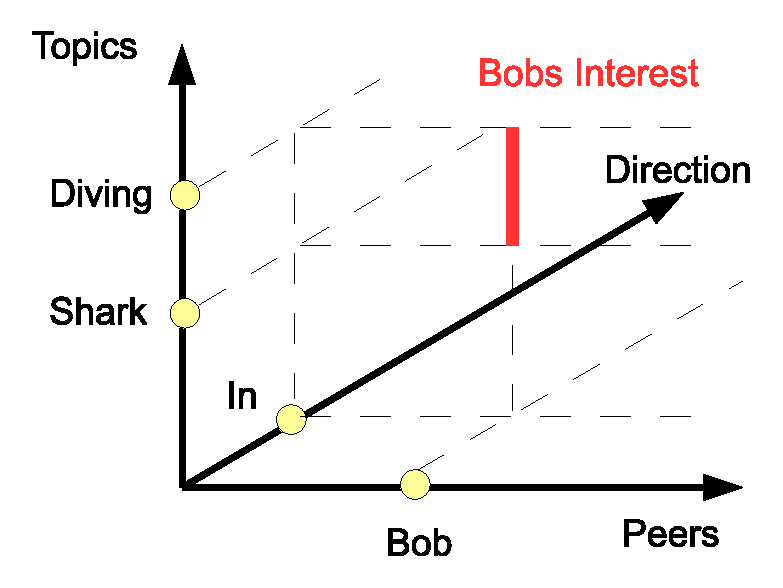
\includegraphics[width=0.60\textwidth]{bobsInterest.eps}
\caption{Bob's Interest}
\label{fig:contextspace}
\end{figure}

Let's have a look at the peer dimension. Bob has defined himself and no other peers. This definition creates a plane in Bobs context space. All point which are not in this plane are not covered by Bobs interest.

Bob has defined two topics. Mathematically, that definition creates two additional planes which subtend our first plane. Two lines are created. Bob has no restrictions in remote peers. We can conclude now: Any point one each of both lines are in Bobs interest.

More abstract but also more accurate: An interest defines a single hyperplane in the seven dimensional context space. An interest describes a point if each dimension is defined by a single tag. Thus, context coordinates can be seen as special interest.

An interest covers the whole context space if each dimension is defined by the any tag. We call it the {\it any interest}.

Note, a point in context space doesn't have necessarily information. A point is just a set of tags defining a context in which information can be stored.

\section{Find information with interests}
Information can be retrieved from a knowledge base by means of interests.
We continue our previous example.

\begin{verbatim}
// create parts of interest
STSet intTopics = InMemoSharkKB.createInMemoSTSet();
PeerSTSet intPeers = InMemoSharkKB.createInMemoPeerSTSet();

// add copy of shark tag
intTopics.merge(shark);
// add diving tag
intTopics.createSemanticTag("Diving", "http://www.diving.de");

intPeers.merge(alice);

// create interest
Interest interest = InMemoSharkKB.createInMemoInterest(
   intTopics, // topics
   null, // don't care originator
   intPeers, // peers
   null, // don't care about remote peers
   null, // don't care about time
   null, // don't care about location
   SharkCS.DIRECTION_OUT); // look for information to be sent

// use it to retrieve information from kb
Enumeration<ContextPoint> cpEnum = kb.getContextPoints(interest);
if(cpEnum != null) {
   System.out.println("found information");
   System.out.println(L.knowledge2String(cpEnum));
}
\end{verbatim}

Interests have seven dimensions. Most of them are sets of semantic tags. In this example we first create two sets. One will contain interesting topics. The other one contains peers. We use 'Shark' and 'diving' as topics and Alice as peer.

We create an interest with our in-memo knowledge base and use it to look for non-empty context points with {\tt getContextPoints()}. An enumeration object is returned if at least one context point can be found with attached information.
We use our logger class {\tt L} to print the results.

The example will find our one and only information. It was found even without explicitly declaring an originator in the interest. It is set to {\tt null} which means {\it any}.

In some circumstances it might be necessary to escape the usage of {\tt null} as {\it any} tag. Sometimes we look for context points in which a dimension is not set. In this case, we can use this code:

\begin{verbatim}
cpEnum = kb.getContextPoints(interest, false);
if(cpEnum != null) {
   System.out.println("found information");
   System.out.println(L.knowledge2String(cpEnum));
} else {
   System.out.println("no information found");
}
\end{verbatim}

We use the variant {\tt getContextPoints(interest, false)}. The second parameter is set to false. This prevents the knowledge base from interpreting undefined dimensions as {\it any tags}. This version looks for context points with unset dimensions in originator, time and location dimension.

This code will produce the output {\tt no information found}.

Note, {\tt getContextPoints(i, true)} is identical to {\tt getContextPoints(i)}.

\subsection{Any tags in interests}
We want to discuss the use of {\it any} tags in interests in more in detail. You can skip that section during first reading. But come back later.

Semantic tags without an explicit meaning are called {\it any} tags in Shark.
We could already see, that coordinates can have an {\it any} tag. Each dimension has -- per definition -- an {\it any} tag. An exception is the direction.

Thus, {\it any} in context coordinates are interpreted as {\it don't know} rather than {\it anything}. Why is that? Authors create coordinates. They know their content. They will hardly state that information fit to any thinkable topic in the world. More likely, they haven't found an appropriate subject identifier.

The problem arises when facing the interests. What is meant if a user declares {\it any} e.g. in topic dimension? From a technical point of view, it could have two meanings:
\begin{enumerate}
    \item The user is interested in information which has no defined topic. The user is not interested in any information with a declared topic.
\item
The user has no constraints in topics.
\end{enumerate}

We have chosen the last interpretation\footnote{And we have already seen that developers can change that decision. There are two variants of {\tt getContextPoints}, see previous section.} as default. Thus, an {\it any tag} in interests declares that dimension to be free of constraints. Anything would fit.

In conclusion, the most general interest is the following one:

(Any, Any, Any, Any, Any, Any, INOUT).

It could be translated in: A peer that doesn't reveal its identity is interested in sending and receiving information about arbitrary topics. It has no constraints on communication partners, locations and time.

This interest isn't as useless as it might look at the first glance. We come back to the point when we talk about mutual interests.

Let's have a look at this interest:

(Tourist information, Any, Any, Any, Berlin, Any, IN).

This interest can be described as: A peer that doesn't reveal its identity wants to receive tourist information in Berlin. It has no further constraints. Looks like a location based service.

Or this one:

(Any, Any, Bob, Alice, Any, Any, INOUT).

Bob is interested in sharing anything with Alice.

\section{Contextualization}
Now we have reached the very core of the Shark data model and even the Shark concept. Shark is about storing information with context and it is about exchanging information.

Information exchange shall be based on {\it mutual interests}. Now we explain how mutual interests can be {\it calculated}. Let's do it with an example first and let's come back to Alice and Bob.

We have already seen that Alice had stored information about Shark and is willing to share it. She stored her information with a knowledge base and used those coordinates which can also be seen and used as interest.\\
(Shark, Alice, Alice, Any, Any, Any, OUT)\\
She (Alice) offers something about Shark to anybody, anywhere and anytime.

A P2P system needs to be at least one other peer. That's Bob. He might be interested in exchange of anything which is of any interest by Alice. Such interest can be described.\\
(Any, Any, Bob, Alice, Any, Any, INOUT).

Note the last dimension {\tt inout}. He wants to send but also receive  information. Lets have a look on a fresh code example that firstly creates both interests.

\begin{verbatim}
// create alice interest
STSet aliceTopics = InMemoSharkKB.createInMemoSTSet();
aliceTopics.createSemanticTag( // create topic shark
   "Shark", // name
   "http://www.sharksystem.net"); // si

// create peer alice
PeerSemanticTag alice = InMemoSharkKB.createInMemoPeerSemanticTag(
            "Alice", // name
            "http://www.sharksystem.net/alice.html", // si
            "mail://alice@wonderland.net"); // address

// create peer tag set
PeerSTSet alicePeers = InMemoSharkKB.createInMemoPeerSTSet();
alicePeers.merge(alice);

// create interest for alice
Interest aliceInterest = InMemoSharkKB.createInMemoInterest(
   aliceTopics, // her topics: shark
   alice, // she offers her information
   alicePeers, // stored in her knowledge base
   null, null, null, // don't care about time, place, remote peers
   SharkCS.DIRECTION_OUT); // offers information

// debugging: print it out.
System.out.println("Alice interest:\n " +
    L.contextSpace2String(aliceInterest));

// let's do it with bob as well
PeerSTSet bobPeers = InMemoSharkKB.createInMemoPeerSTSet();
bobPeers.createPeerSemanticTag("Bob", // name
            "http://www.sharksystem.net/bob.html", // si
            "mail://bob@wonderland.net"); // address

PeerSTSet bobRemotePeers = InMemoSharkKB.createInMemoPeerSTSet();
bobRemotePeers.merge(alice); // wants to talk with Alice only

Interest bobInterest = InMemoSharkKB.createInMemoInterest(
   null, null, // topic and originator irrelevant
   bobPeers, // that's bob
   bobRemotePeers, // only alice
   null, null, // don't care about time and place
   SharkCS.DIRECTION_INOUT); // sending, receiving

// debugging: print it out
System.out.println("Bob interest:\n " +
    L.contextSpace2String(bobInterest));
\end{verbatim}

Interests are defined by peers. Interests can be sent. Let's assume that Alice has received Bobs interest. For us it is very simple to find the mutual interest. If Bob wants to share anything with Alice and Alice offers information about java to anybody it is obvious: Both have the interest, that Alice sends information about Java to Bob anywhere and anytime.

(Shark, Alice, Alice, Bob, Any, Any, OUT)

Let's have a closer look at the calculation: Bob had no constraints about the topic. Alice did: The intersection of both is Shark. Bob had no constraints regarding originator. Alice did. The intersection is Alice.

Bob has introduced himself as Bob in peer dimension. So did Alice. She introduced herself as Alice. Apparently, Alice should not try to find out if both  {\it peer} dimensions fit. She should try to find out if peer in received interest fits to her constraints about remote peers - and vice versa.

Alice had no constraints about remote peers, Bob only wants to talk with Alice. The intersection is Bob. Alice is making that calculation and Bob is the remote peer.

Bob has constraints about his remote peers: He only wants to talk with Alice. Alice has revealed her identity - that fits. Alice is put into the peer dimension.

Both peers have no constraints in location and time. There are no constraints in the mutual interests either. Bob wants to communicate in both directions. Alice only wants to send.

This sound complicated and actually it is. The good new is - Shark makes those calculations for you:

\begin{verbatim}
// zero fp: don't follow any relation. depth = 0
FragmentationParameter fp = FragmentationParameter.getZeroFP();

//use that fp for each dimension
FragmentationParameter[] fps = new
   FragmentationParameter[SharkCS.MAXDIMENSIONS];

for(int d = 0; d < SharkCS.MAXDIMENSIONS; d++) {
   fps[d] = fp;
}

// calculate mutual interest
Interest mutualInterest = SharkCSAlgebra.contextualize(
   bobInterest, // source - the received interest
   aliceInterest, // context - the local interest
   fps);

// watch the result
System.out.println("Alice calculates: Bob / Alice:\n " +
    L.contextSpace2String(mutualInterest));

\end{verbatim}

Imagine, Bob would receive Alice's interest. He could do the same calculation and would come to that result:

(Java, Alice, Bob, Alice, Any, Any, IN)

That result differs in three points: peer, remote peer and direction. And that's only logical. We are on Bobs side now. Bob puts himself into the peer dimension and Alice in the remote peer slot of course. He also learnt that Alice only wants to send something, so he changed the direction to IN.

We extend our program with those lines:
\begin{verbatim}
mutualInterest = SharkCSAlgebra.contextualize(
   aliceInterest, // source - received interest
   bobInterest, // context - local interest
   fps);

System.out.println("Bob calculates: Alice / Bob:\n " +
   L.contextSpace2String(mutualInterest));
\end{verbatim}

Both mutual interests describe a potential information exchange. Both mutual interests differ because they describe the same exchange from different perspectives.

Bob describes Alice as {\it remote peer} and vice versa. Alice describes an interest in {\it sending} information. This fits to Bob because he wants also to {\it receive} information. Once an interest is received it has to be translated into the recipient peers perspective.

We have used our algebra class {\tt SharkCSAlgebra} for our calculation. Applying {\tt contextualize} on {\tt interest} automatically makes the translation of perspective. The method takes three parameters. First is a {\it source} which is meant to be the received interest. Second parameter is the {\it context} which is meant to be the interest created by the receiving peer.

The fragmentation parameter are used for those calculations. The algorithm is explained in detail in next sub section.

Does it sound complicated even irritating? Don't panic! The good news is that most applications don't have to deal with those details. Everything is already implemented and there are already predefined and implemented classes that perform the information exchange that fits to a huge number of applications (namely {\tt StandardKP}).

Have a look on the algorithm if you like. It is not necessary when first reading this book. Read it if you run into problems in your applications.

\subsubsection{Algorithm}
The algorithm explanation is a brief one compared to the motivation. We already know contextualisation in semantic tag sets. The context space contextualisation algorithm works as described below.

\begin{enumerate}
    \item The Algorithm has two parameter: Source and context. Both are context spaces. A third context space will be the result -- we call it fragment.
\item The topic dimension in the fragment is created by means of a contextualisation of two semantic tag sets. The source set is the topic dimension of source and the context set is the topic dimension of the context.
\item The same operation is made with location and time. Source location and time is contextualised with context location and time.
\item The sources originator is contextualised with the contexts originator.
\item
The fragment peer dimension is the result of the contextualisation of the sources remote peer dimension with the contexts peer dimension.
\item
The fragments remote peer dimension is the result of the contextualisation of the sources peer dimension with the contexts remote peer dimension.
\item
The contextualisation of the direction differs from the calculations above and is explained in table \ref{tab:directionCalculation}
\end{enumerate}

\begin{table}[t]
\centering
\begin{tabular}{|c|c|c|}
\hline
Source & Context & Fragment \\
\hline
INOUT & INOUT & INOUT \\
\hline
INOUT & OUT & OUT \\
\hline
INOUT & IN & IN \\
\hline
OUT & INOUT & NON \\
\hline
OUT & OUT & NON \\
\hline
OUT & IN & IN \\
\hline
IN & INOUT & OUT \\
\hline
IN & OUT & OUT \\
\hline
IN & IN & NON \\
\hline
NON & * & NON \\
\hline
* & NON & NON \\
\hline
\end{tabular}
\caption{Direction contextualisation}
\label{tab:directionCalculation}
\end{table}

\section{Other operations}

\subsection{Is in}
The context space describes a sub space. A point can be in the sub space or not.
There is a method that checks whether a point described by context coordinates is within or outside a sub space.

The actual algorithm is straightforward: Most of each context space dimension is described with a set of semantic tags. Each possible combination of coordinates is created. The point is in the context space if one combination fits with the given coordinates.

Let's have an example. We choose just two dimensions to shorten the description.

Lets have a two dimensional space constituted by topic and peer. Lets define a point with the dimension ({\it Java}, {\it Alice}). Lets define a context space:
({\it (Java, Skiing), (Alice, Bob)}). Is the point inside the context space?

The figure \ref{fig:csIsIn} shows the context space and the point (Java, Alice):

We create any possible point inside the context space which are four in our example:\\
{\it (Java, Alice)}\\
{\it (Java, Bob)}\\
{\it (Skiing, Alice)}\\
{\it (Skiing, Bob)}\\

Those four points are the whole context space. Just four points -- nothing more. It is a discrete space -- there is nothing {\it between} Alice and Bob or Java and Skiing. Apparently, the point ({\it Java}, {\it Alice}) is part of the context space.

\begin{figure}[t]
\centering
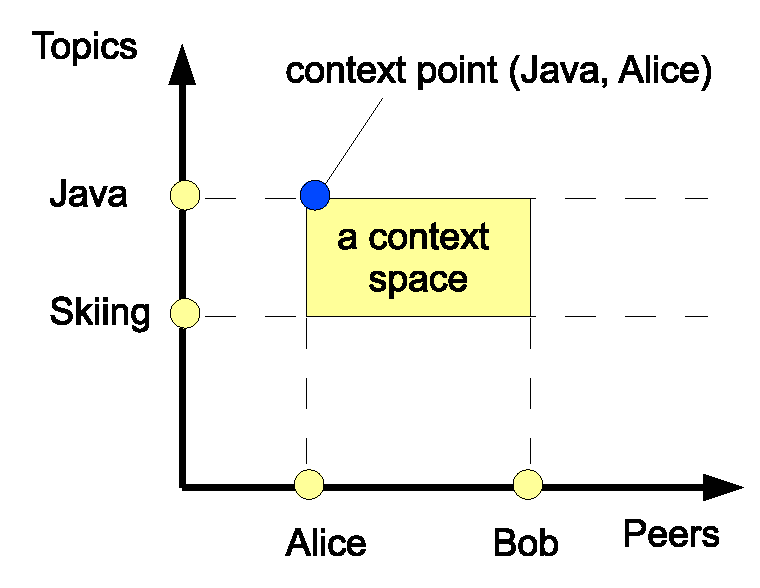
\includegraphics[width=0.60\textwidth]{insideAContextSpace.eps}
\caption{Inside a Context Space}
\label{fig:csIsIn}
\end{figure}

The following code creates an interest, coordinates and performs the test.

\begin{verbatim}

SemanticTag skiing =
   InMemoSharkKB.createInMemoSemanticTag(
         "Skiing", "http://www.skiing.de");

SemanticTag java = InMemoSharkKB.createInMemoSemanticTag(
         "Java", "http://www.java.de");

PeerSemanticTag alice =
   InMemoSharkKB.createInMemoPeerSemanticTag(
      "Alice", // name
      "http://www.sharksystem.net/alice.html", // si
      "mail://alice@wonderland.net"); // address

PeerSemanticTag bob =
   InMemoSharkKB.createInMemoPeerSemanticTag(
     "Bob", // name
     "http://www.sharksystem.net/bob.html", // si
     "mail://bob@wonderland.net"); // address

// create interest (context space)
STSet topics = InMemoSharkKB.createInMemoSTSet();
topics.merge(skiing);
topics.merge(java);

PeerSTSet peers = InMemoSharkKB.createInMemoPeerSTSet();
peers.merge(alice);
peers.merge(bob);

Interest interest = InMemoSharkKB.createInMemoInterest(
   topics, null, peers, null, null, null,
   SharkCS.DIRECTION_INOUT);

System.out.println("interest:\n " +
    L.contextSpace2String(interest));

// create coordinates
ContextCoordinates cc =
   InMemoSharkKB.createInMemoContextCoordinates(
      java, null, alice, null, null, null,
      SharkCS.DIRECTION_INOUT);

System.out.println("CC:\n" + L.contextSpace2String(cc));

if(SharkCSAlgebra.isIn(interest, cc)) {
   System.out.println("is in");
} else {
   System.out.println("is in");
}
\end{verbatim}

\subsection{Identical}
Two context spaces are defined to be identical if both comprises the same points.
We could also say that each point of context A must by {\it in} context B and vice versa. We could also say that all context space dimensions must be identical. That method is simple and so is the code. We extend the previous code.

\begin{verbatim}
if(!SharkCSAlgebra.identical(interest, cc)) {
   System.out.println("Not identical");
}
\end{verbatim}

\section{Context Space interfaces}
Figure \ref{fig:contextSpaceHierarchy} illustrates most important interfaces which make up context space in Shark.

{\tt ContextSpace} just defines the basic fact that a context space is made up by dimensions. {\tt SharkCS} defines number and names of dimensions and some basic methods and important constants. What is {\tt ContextSpace} good for?

It is a heritage and a reminder. There is a more generic theory on context space explained in my PhD. Context spaces is a general concept for independent and co-operating knowledge bases. The number of dimensions is irrelevant for the more general concept. Those, there could be implementations that don't use seven dimensions but an arbitrary other number of dimensions and dimension types.

{\tt SharkCS} describes the Shark context space. It makes clear, that Shark uses seven dimensions with the defined semantics. {\tt SharkCSAlgebra} implements all algorithms for this seven dimensional incarnation. Some classes also offer methods like {\tt contextualization} and {\tt fragmentation}. Finally, any of those methods use this central class. We suggest to use the algebra class whenever possible.

{\tt ContextCoordinates} and {\tt Interests} are derived from {\tt SharkCS} and define point and hyperplane in the context space.

\begin{figure}[t]
\centering
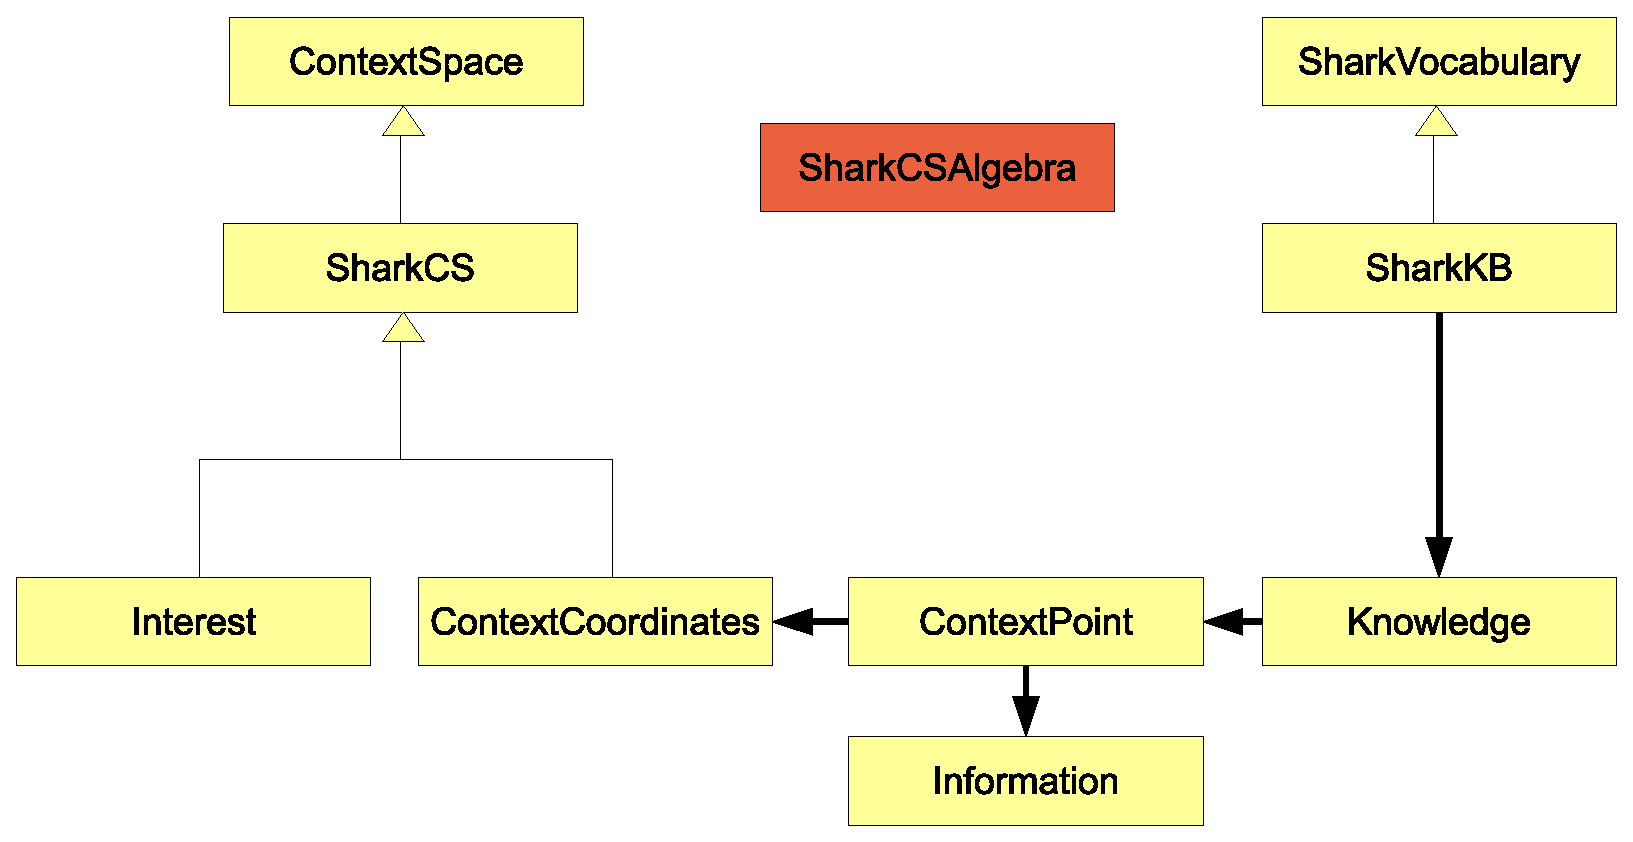
\includegraphics[width=0.90\textwidth]{CSInterfaces.eps}
\caption{Most relevant Context Space Classes and Interfaces}
\label{fig:contextSpaceHierarchy}
\end{figure}

All those interfaces are implemented with a knowledge base implementation which will be discussed next chapter. A knowledge base stores tags, tags sets and information in a context space. A knowledge base is more than a context space but it can be used as context space ({\tt SharkKB.asSharkCS()}). But that's already topic of the next chapter.

\section{Exercises}
\begin{enumerate}
\item
Given following vocabulary. Create a cs..
\item
Add information to the given point in cs.
\item
write some examples and ask reader to change it..
\end{enumerate}
